\section{Resultados}

Definida e implementada toda a arquitetura do projeto, chegou-se a
resultados finais satisfatórios, tendo sido implementadas todas as
primitivas de forma bem sucedida.\newline
\break
\noindent
Os resultados a que se chegou podem, então ser observados nas Figuras
\ref{fig:planefinal}, \ref{fig:boxfinal}, \ref{fig:spherefinal}
e \ref{fig:conefinal}.

\subsection{Plano}

\begin{center}
    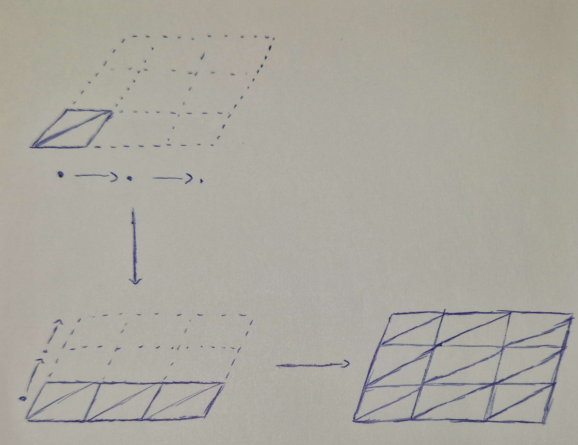
\includegraphics[width=0.8\textwidth]{imgs/plane.png}
    \captionof{figure}{Plano implementado}
    \label{fig:planefinal}
\end{center}

\subsection{Caixa}

\begin{center}
    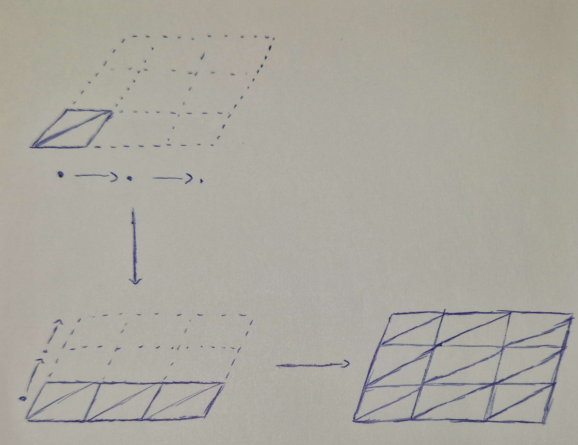
\includegraphics[width=0.8\textwidth]{imgs/plane.png}
    \captionof{figure}{Caixa implementada com far pequeno}
    \label{fig:boxfinal}
\end{center}

\subsection{Esfera}

\begin{center}
    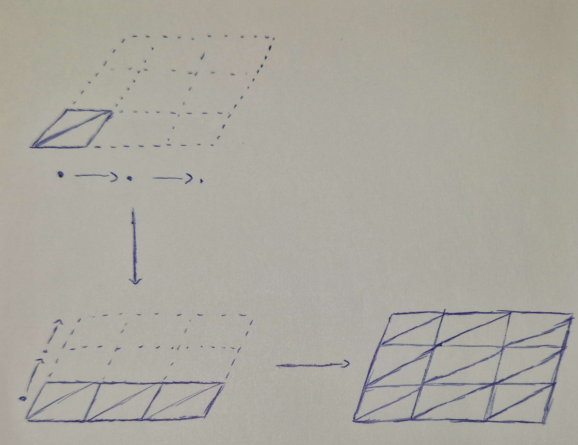
\includegraphics[width=0.8\textwidth]{imgs/plane.png}
    \captionof{figure}{Esfera implementada}
    \label{fig:spherefinal}
\end{center}

\subsection{Cone}

\begin{center}
    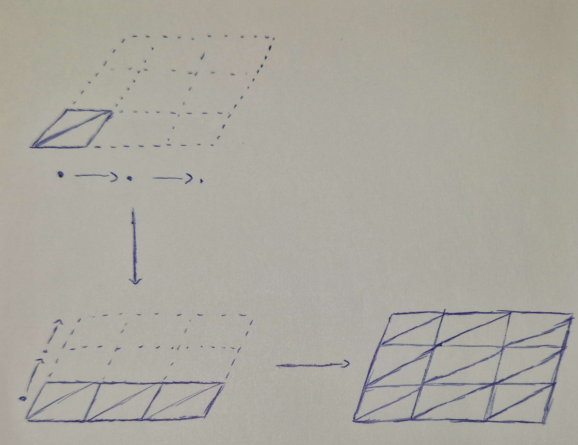
\includegraphics[width=0.8\textwidth]{imgs/plane.png}
    \captionof{figure}{Cone implementado}
    \label{fig:conefinal}
\end{center}